\documentclass{apuntes}

\title{Automatas y lenguajes}
\author{Pedro Valero}
\date{14/15 C1}

% Paquetes adicionales

% --------------------

\begin{document}
\pagestyle{plain}
\maketitle

\tableofcontents
\newpage

\printindex

\chapter{Introducción}
Vamos a trabajar con tres elementos fundamentales:
\begin{itemize}
\item \textbf{Máquinas/Autómata}
\begin{itemize}
\item Autómatas finitos $\Rightarrow$ Expresiones regulares
\item Autómatas de pila $\Rightarrow$ Lenguajes libres de contexto
\end{itemize}
\item \textbf{Problemas} ¿Qué se puede computar?. Conjeturas que se creen ciertas pero cuya veracidad, por ahora, no se ha demostrado.

\item \textbf{Lenguajes/Gramática}
\end{itemize}

Nuestro objetivo es ver que relacion existe entre estos tres elementos. Para ello, primero debemos establecer algunas definiciones.

\section{Lenguaje}
\begin{defn}[Símbolo]
``Letra", elemento de un conjunto
\end{defn}

\begin{defn}[Alfabeto]
Conjunto finito de símbolos no vacío.
\end{defn}

\begin{defn}[Palabra (Cadena)]
Secuencia finita de símbolos tomados de un alfabeto.
La palabra vacía se representa por $\lambda$
\end{defn}
Será conveniente acostumbrarnos a usar el término ``cadena" en lugar del término ``palabra" ya que representa mejor el concepto que queremos representar.


\begin{defn}[Longitud de cadena]
Número de símbolos que contiene
\end{defn}

\begin{defn}[Lenguaje]
Conjunto de palabras
\end{defn}

Hay algunos casos particulares de lenguajes:
\subsection{Lenguajes particulares}
\begin{defn}[Lenguaje universal (sobre $\sum$)]
Denotado por $\sum^*$ representa el conjunto de todas las palabras que se pueden formar
\end{defn}

\begin{defn}[Lenguaje de un autómata]
Conjunto de palabras que acaban en un estado final del autómata son aceptadas por el mismo)
\end{defn}

\begin{defn}[Lenguaje vacío]
Lenguaje que no contiene ningún elemento
\end{defn}

\begin{defn}[Lenguaje $\lbrace \lambda \rbrace$]
Lenguaje que sólo contiene $\lambda$.
\end{defn}
El lenguaje $\lbrace \lambda \rbrace$ es distinto del lenguaje vacío aunque $\lambda$ sea la palabra vacía.

\section{Gramática}
\begin{defn}[Gramática]
Hay varias definiciones para este término. No son muy precisas pero nos dan una idea de su significado:
\begin{enumerate}
\item Mecanmismo para formalizar matemáticamente un lenguaje
\item Conjunto de reglas que determinan cómo formar las cadenas de un lenguaje
\end{enumerate}
\end{defn}

\begin{example}
Tomemos las reglas:
\begin{enumerate}
\item ORACIÓN $\Rightarrow$ SUJETO + PREDICADO
\item SUJETO $\Rightarrow$ ARTÍCULO + NOMBRE
\item PREDICADO $\Rightarrow$ VERBO
\item ARTÍCULO $\Rightarrow$ el ó un
\item NOMBRE $\Rightarrow$ coche ó perro
\item VERBO $\Rightarrow$ come ó correo
\end{enumerate}
Estas reglas constituyen una gramática que nos permite generar un lenguaje. En este caso el lenguaje estaría formado todas las cadenas que se pueden construir a partir de estas reglas
%TODO Ejemplo de árbol de derivación con estas reglas
\end{example}

\begin{defn}[Símbolos terminales]
Símbolos que pueden aparecer en la cadena final. En el ejemplo anterior serían elementos terminales aquellos escritos en minúscula. Para ellos no existe ninguna regla que indique cómo se derivan.
\end{defn}

\begin{defn}[Símbolos no terminales]
Símbolos que no pueden aparecer en la cadena final. Simplemente son usados para definir las reglas de derivación
\end{defn}

\begin{defn}[Reglas de producción]
Explican cómo se transforma un símbolo no terminal en un conjunto de símbolos terminales o no terminales
\end{defn}

\begin{defn}[Símbolo inicial / Axioma]
Indica dónde empieza a construirse la cadena. En el ejemplo anterior, el axioma sería el símbolo ORACIÓN. Una gramática sólo puede tener un úncio axioma.
\end{defn}

Vamos a ver algunos ejemplos de gramáticas y los lenguajes que generan:
\begin{example}
Tomemos la gramática:
\begin{enumerate}
\item S $\Rightarrow$ aSb
\item S $\Rightarrow$ $\lambda$
\end{enumerate}

El lenguaje generado por esta gramática serían todas las palabras de la forma: $a^i\lambda b^i$ con $ i=0,1,... \infty$
\end{example}

\begin{example}
Ahora vamos a tratar de construir la gramática que define un lenguaje dado:
L(G)=$\lbrace a^nb^{n+1}, n \geq 0 \rbrace$

La gramática que define este lenguaje es:
Tomemos la gramática:
\begin{enumerate}
\item S $\Rightarrow$ aSb
\item S $\Rightarrow$ b
\end{enumerate}

El automata asociado a este lenguaje sería:
\begin{center}
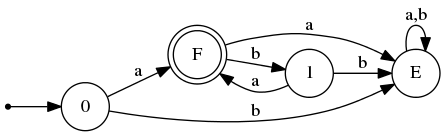
\includegraphics[scale=0.75]{automata1.png}
\end{center}
\end{example}

\begin{defn}[Lenguajes Regulares]
Son lenguajes que pueden ser admitidos por autómatas finitos
\end{defn}

\begin{defn}[Gramáticas libres de contexto]
Son aquellas donde a la izquierda sólo aparece un único símbolo no terminal
\end{defn}


\begin{example}[Gramática dependiente de contexto]
\begin{itemize}
\item aSb $\Rightarrow$ abb
\item cSd $\Rightarrow$ cdd
\end{itemize}
S puede derivarse dependientemente de lo que la rodee, es decir, de su contexto
\end{example}

\begin{example}[Gramática independiente de contexto (regular)]
\begin{itemize}
\item A $\Rightarrow$ aA
\item A $\Rightarrow$ a
\end{itemize}
A la derecha tenemos únicamente símbolos terminales o bien símbolos terminales acompañados de un único símbolo no terminal.
Si el elemento no terminal está a la izquierda se denomina gramática lineal por la derecha. En caso contrario, gramática lineal por la izquierda
\end{example}

\begin{defn}[Equivalencia de gramáticas]
Dos gramáticas son equivalentes si generan el mismo lenguaje
\end{defn}
\end{document}
